\documentclass[tikz]{standalone}

\begin{document}

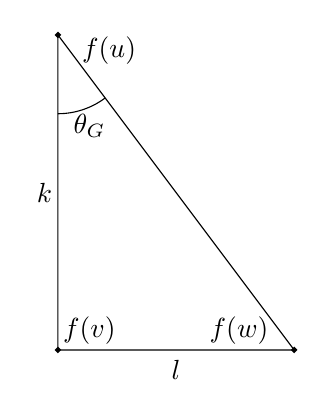
\begin{tikzpicture}

  \node at (0, 0) [circle,inner sep=0pt,line width=1pt,minimum size=1pt,draw] {};
  \node at (0, 4) [circle,inner sep=0pt,line width=1pt,minimum size=1pt,draw] {};
  \node at (3, 0) [circle,inner sep=0pt,line width=1pt,minimum size=1pt,draw] {};

  \draw (0,0) -- (0,4) -- (3,0)-- (0,0);
  \draw (0,3) arc (-90:-53.13010235415598:1);
  \draw (0.4, 2.85) node{$\theta_G$};
  \draw (0.65, 3.8) node{$f(u)$};
  \draw (0.4, 0.25) node{$f(v)$};
  \draw (2.3, 0.25) node{$f(w)$};

  \draw (-0.17, 2) node{$k$};
  \draw (1.5, -0.25) node{$l$};

\end{tikzpicture}

\end{document}
